\chapter{Modular Forms and L Functions for Probabilists}\label{ch:02}

In 1916 Srinivasa Ramanujan published a paper on certain arithmetical functions \cite{ramanujan1916} in which he studied the coefficients $\tau(n)$ of the power series $q\prod_{n\ge1}(1-q^n)^{24}$. From a table of thirty values he guessed three properties: $\tau$ is multiplicative, it satisfies a second order recursion at prime powers, and $|\tau(p)|\le2p^{11/2}$. Mordell proved the first two a year later \cite{mordell1917}; the third waited until Deligne's proof of the Weil conjectures in 1974 \cite{deligne1974}. Hecke's theory of operators on modular forms explains the first two observations, and the third is the prototype of the Ramanujan conjecture for automorphic representations. This chapter develops the objects of that story for readers whose training is in probability: modular forms, Hecke operators, Euler products, Mellin transforms and functional equations. Along the way we isolate two facts that drive the later parts of the book: by Deligne's theorem the normalised Hecke eigenvalues are traces of elements of $\SU(2)$, and the completed $L$ function of $\Delta$ is the Mellin transform of a \emph{positive} function.

\section{The modular group and modular forms}\label{sec:02forms}

The group $\SL_2(\Z)$ of integer matrices of determinant one acts on the upper half plane $\mathbb H=\{\tau\in\C:\Im\tau>0\}$ by M\"obius transformations
\[
\gamma\tau=\frac{a\tau+b}{c\tau+d},\qquad\gamma=\begin{pmatrix}a&b\\c&d\end{pmatrix}\in\SL_2(\Z),
\]
and $\Im(\gamma\tau)=\Im\tau/|c\tau+d|^2$. The group is generated by the matrices $T$ and $S$ that act by $\tau\mapsto\tau+1$ and $\tau\mapsto-1/\tau$, and every orbit meets the closed fundamental domain $\mathcal F=\{\tau\in\mathbb H:|\Re\tau|\le\tfrac12,\ |\tau|\ge1\}$. The quotient $\SL_2(\Z)\backslash\mathbb H$ has finite hyperbolic area $\pi/3$ for the measure $dx\,dy/y^2$, where $\tau=x+iy$, so $\frac3\pi\,dx\,dy/y^2$ is a probability measure on it; it is the limit law of Heegner points in Chapter~\ref{ch:11b}.

\begin{definition}\index{modular form}
Let $k$ be an even integer. A \emph{modular form} of weight $k$ for $\SL_2(\Z)$ is a holomorphic function $f$ on $\mathbb H$ with
\[
f(\gamma\tau)=(c\tau+d)^kf(\tau)\qquad\text{for all }\gamma\in\SL_2(\Z),
\]
which is holomorphic at infinity in the following sense. Invariance under $T$ gives a Fourier expansion $f(\tau)=\sum_{n\in\Z}a(n)q^n$ in $q=e^{2\pi i\tau}$, and we require $a(n)=0$ for $n<0$. If also $a(0)=0$, $f$ is a \emph{cusp form}. The spaces are $M_k$ and $S_k$.
\end{definition}

Invariance under $S$ is the nontrivial condition: $f(-1/\tau)=\tau^kf(\tau)$. The spaces are finite dimensional: for even $k\ge0$, $\dim M_k=\lfloor k/12\rfloor+1$ unless $k\equiv2\bmod12$, in which case $\dim M_k=\lfloor k/12\rfloor$, and $\dim S_k=\dim M_k-1$ for $k\ge4$ \cite{serre1973}. In particular $S_k=0$ for $k<12$ and for $k=14$, and $\dim S_{12}=1$.

\subsection{Eisenstein series}
\index{Eisenstein series}
For even $k\ge4$ the series $\sum_{(c,d)\neq(0,0)}(c\tau+d)^{-k}$ converges absolutely and is visibly of weight $k$. Normalised to have constant term one it becomes
\[
E_k(\tau)=1-\frac{2k}{B_k}\sum_{n\ge1}\sigma_{k-1}(n)q^n,\qquad\sigma_{k-1}(n)=\sum_{d\mid n}d^{k-1},
\]
with $B_k$ the Bernoulli numbers. Thus $E_4=1+240\sum\sigma_3(n)q^n$ and $E_6=1-504\sum\sigma_5(n)q^n$. The coefficients $\sigma_{k-1}(n)$ are multiplicative, and at a prime $\sigma_{k-1}(p)=1+p^{k-1}$. This is the degenerate case of everything that follows. The form $E_k$ is an eigenvector of the Hecke operator $T_p$ of the next section with eigenvalue $\sigma_{k-1}(p)$; the roots of $X^2-\sigma_{k-1}(p)X+p^{k-1}$ are $1$ and $p^{k-1}$, and after division by $p^{(k-1)/2}$ they are $p^{\pm(k-1)/2}$, far from the unit circle. The normalised eigenvalues $p^{(k-1)/2}+p^{-(k-1)/2}$ are unbounded, so they are not traces of elements of a compact subgroup of $\GL_2(\C)$: equidistribution in a compact group, the probabilistic shadow of Chapter~\ref{ch:01}, is a phenomenon of cusp forms.

\subsection{Ramanujan's Delta}
\index{Ramanujan Delta function}
The normalised cusp form of weight $12$ is
\[
\Delta(\tau)=\frac{E_4(\tau)^3-E_6(\tau)^2}{1728}=q\prod_{n\ge1}(1-q^n)^{24}=\sum_{n\ge1}\tau(n)q^n=\eta(\tau)^{24},
\]
where $\eta(\tau)=q^{1/24}\prod_n(1-q^n)$ is the Dedekind eta function\index{Dedekind eta function}. The equality of the Eisenstein expression with the product is Jacobi's; it can be proved by checking that the product is a cusp form of weight $12$, using the transformation law $\eta(-1/\tau)=\sqrt{\tau/i}\,\eta(\tau)$, and comparing the first coefficient.

\begin{example}\label{ex:02tau}
Expanding $q(1-q)^{24}(1-q^2)^{24}(1-q^3)^{24}\cdots$ to order $q^4$: the coefficient of $q^2$ comes only from $(1-q)^{24}$ and is $\tau(2)=-24$. The coefficient of $q^3$ receives $\binom{24}{2}=276$ from $(1-q)^{24}$ and $-24$ from $(1-q^2)^{24}$, so $\tau(3)=252$. For $q^4$ we collect $-\binom{24}{3}=-2024$ from $q^3$ in $(1-q)^{24}$, then $(-24)\cdot(-24)=576$ from $q\cdot q^2$, and $-24$ from $q^3$ in $(1-q^3)^{24}$, so $\tau(4)=-2024+576-24=-1472$. Continuing, $\tau(5)=4830$ and $\tau(6)=-6048=\tau(2)\tau(3)$.
\end{example}

\begin{theorem}[Ramanujan's observations]\label{thm:02ramanujan}
The coefficients $\tau(n)$ satisfy:
\begin{enumerate}
\item $\tau(mn)=\tau(m)\tau(n)$ when $\gcd(m,n)=1$ (Mordell, 1917);
\item $\tau(p^{r+1})=\tau(p)\tau(p^r)-p^{11}\tau(p^{r-1})$ for primes $p$ and $r\ge1$ (Mordell, 1917);
\item $|\tau(p)|\le2p^{11/2}$ for all primes $p$ (Deligne \cite{deligne1974}).
\end{enumerate}
\end{theorem}

The first two follow from the theory of Hecke operators in the next section, since $\Delta$ spans the one dimensional space $S_{12}$. The third follows from the Weil conjectures, which Deligne proved, applied to a Kuga Sato variety: a smooth compactification of the tenth fibre power of the universal elliptic curve (with auxiliary level structure), a variety of dimension $11$ in whose cohomology $\tau(p)$ is the trace of Frobenius on a two dimensional piece of $H^{11}$ \cite{deligne1971}. Example~\ref{ex:02tau} checks (2) at $p=2$, $r=1$: $\tau(2)^2-2^{11}=576-2048=-1472=\tau(4)$.

Whether $\tau(n)$ is ever zero is a question Lehmer raised in 1947 \cite{lehmer1947}, still open. Lehmer showed that the least $n$ with $\tau(n)=0$, if any, is prime; computations of Derickx, van Hoeij and Zeng \cite{derickx2013} based on congruences for $\tau$ have shown that $\tau(n)\neq0$ for all $n$ below $8\times10^{23}$. Serre proved that the primes with $\tau(p)=0$ have density zero \cite{serre1981}. Lehmer's question is the weight $12$ analogue of the Lang Trotter question for the trace $t=0$ (Chapter~\ref{ch:05}). If $\tau(p)/p^{11/2}$ behaved like an independent draw from the Sato Tate law of Chapter~\ref{ch:01}, rounded to the lattice $p^{-11/2}\Z$, the event $\tau(p)=0$ would have probability of order $p^{-11/2}$, a summable sequence. The same heuristic gives probability of order $p^{-1/2}$ for $a_p=0$ on an elliptic curve and so predicts infinitely many supersingular primes; for $\Delta$ it predicts only finitely many zeros of $\tau(p)$, and probably none.

\section{Hecke operators}
\index{Hecke operator}
For a prime $p$ the Hecke operator $T_p$ on $M_k$ sums $f$, viewed as a function of lattices, over the $p+1$ sublattices of index $p$. In coordinates,
\[
(T_pf)(\tau)=p^{k-1}f(p\tau)+\frac1p\sum_{j=0}^{p-1}f\Bigl(\frac{\tau+j}{p}\Bigr),
\]
and on $q$ expansions
\[
a(T_pf,n)=a(np)+p^{k-1}a(n/p),
\]
where $a(n/p)=0$ if $p\nmid n$. The operators $T_n$ for all $n\ge1$ are defined similarly by summing over sublattices of index $n$, and satisfy:

\begin{proposition}[Hecke relations]\label{prop:02hecke}
The operators $T_n$ commute, $T_{mn}=T_mT_n$ for coprime $m,n$, and for each prime $p$ and $r\ge1$,
\[
T_pT_{p^r}=T_{p^{r+1}}+p^{k-1}T_{p^{r-1}}.
\]
\end{proposition}

\begin{proof}[Proof sketch]
Identify $f$ with the function $F(\Z\omega_1+\Z\omega_2)=\omega_2^{-k}f(\omega_1/\omega_2)$ of lattices, where $\Im(\omega_1/\omega_2)>0$; it satisfies $F(\lambda L)=\lambda^{-k}F(L)$, and $T_n$ becomes $T_nF(L)=n^{k-1}\sum_{[L:L']=n}F(L')$. Coprime indices factor uniquely through intermediate lattices, which gives multiplicativity. For the prime power relation, count pairs $L''\subset L'\subset L$ with $[L:L']=p$ and $[L':L'']=p^r$: each sublattice $L''$ of index $p^{r+1}$ arises once unless $L''\subset pL$, in which case it arises $p+1$ times. The excess $p$ copies of each sublattice of $pL$ of index $p^{r-1}$ in $pL$ give the term $p^{k-1}T_{p^{r-1}}$ after the weight normalisation, since $F(pL)=p^{-k}F(L)$. Commutativity follows, since each $T_n$ is then a polynomial in the $T_p$ with $p\mid n$, and $T_pT_q=T_{pq}=T_qT_p$ for primes $p\neq q$. Details are in \cite{serre1973}.
\end{proof}

The relation at a prime is a three term recursion, the same one satisfied by Chebyshev polynomials. If $f$ is a simultaneous eigenvector of all $T_n$ with $a(1)=1$, an \emph{eigenform}, then $a(n)$ is the eigenvalue of $T_n$ (compare the coefficients of $q$ on both sides of $T_nf=\lambda_nf$, using $a(T_nf,1)=a(n)$), and the Hecke relations become
\[
a(mn)=a(m)a(n)\quad(\gcd(m,n)=1),
\]
\[
a(p^{r+1})=a(p)a(p^r)-p^{k-1}a(p^{r-1}).
\]
Since $S_{12}$ is one dimensional, $\Delta$ is an eigenform and Theorem~\ref{thm:02ramanujan}(1),(2) follow.

\subsection{Euler products and Satake parameters}
\index{Satake parameter}
Let $f$ be an eigenform, put $x_p=a(p)/p^{(k-1)/2}$, and let $\alpha_p,\beta_p$ be the roots of $X^2-x_pX+1$, so that $a(p)=p^{(k-1)/2}(\alpha_p+\beta_p)$ and $\alpha_p\beta_p=1$. The recursion becomes
\[
\frac{a(p^r)}{p^{r(k-1)/2}}=\frac{\alpha_p^{r+1}-\beta_p^{r+1}}{\alpha_p-\beta_p}=U_r(x_p/2),
\]
by induction, since the Chebyshev polynomials $U_r$ of the second kind satisfy $U_{r+1}(x/2)=xU_r(x/2)-U_{r-1}(x/2)$; the middle term is read as $(r+1)\alpha_p^r$ when $\alpha_p=\beta_p$. Multiplicativity and the generating function $\sum_{r\ge0}U_r(x/2)t^r=(1-xt+t^2)^{-1}$ give, where the series converges absolutely (for $\Re s>k/2+1$ by Hecke's bound in Section~\ref{sec:02mellin}),
\begin{align*}
L(s,f)=\sum_{n\ge1}\frac{a(n)}{n^s}&=\prod_p\bigl(1-a(p)p^{-s}+p^{k-1-2s}\bigr)^{-1}\\
&=\prod_p\bigl(1-\alpha_pp^{\frac{k-1}2-s}\bigr)^{-1}\bigl(1-\beta_pp^{\frac{k-1}2-s}\bigr)^{-1},
\end{align*}
an Euler product of degree two. The pair $\{\alpha_p,\beta_p\}$ is the Satake parameter, the conjugacy class of $\mathrm{diag}(\alpha_p,\beta_p)$ in $\SL_2(\C)$. Since $a(p)$ is real ($T_p$ is self adjoint for the Petersson inner product of Section~\ref{sec:02level}), Deligne's bound $|a(p)|\le2p^{(k-1)/2}$ is equivalent to $|\alpha_p|=|\beta_p|=1$, that is, to $\alpha_p=e^{i\theta_p}$, $\beta_p=e^{-i\theta_p}$ with $\theta_p\in[0,\pi]$, and then
\[
x_p=\frac{a(p)}{p^{(k-1)/2}}=2\cos\theta_p\in[-2,2].
\]
In probabilistic language: the Satake parameter is a conjugacy class in $\SU(2)$, the normalised eigenvalue $x_p$ is its trace, and the normalised coefficient $a(p^r)/p^{r(k-1)/2}=U_r(x_p/2)$ is the character of $\Sym^r$ evaluated on it. The Sato Tate law, a theorem for $\Delta$ (Theorem~\ref{thm:01satotate}), says that the $\theta_p$ are equidistributed with respect to $\frac2\pi\sin^2\theta\,d\theta$ on $[0,\pi]$, the law of the angle of a Haar random element of $\SU(2)$; equivalently, the $x_p$ are equidistributed with respect to $\ST$.

Figure~\ref{fig:tau} shows this for $\Delta$ and the primes below $10^6$; Chapter~\ref{ch:05} measures the fit by moments (Table~\ref{tab:05moments}), extreme values and discrepancy.

\begin{figure}[t]
\centering
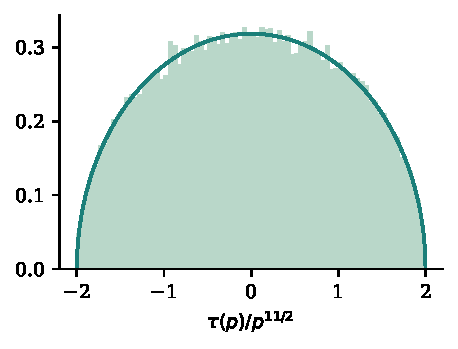
\includegraphics[width=\textwidth]{figs/tau.pdf}
\caption{Histogram of the normalised Ramanujan coefficients $x_p=\tau(p)/p^{11/2}$ for the $78{,}498$ primes $p<10^6$, against the Sato Tate density $\frac1{2\pi}\sqrt{4-x^2}$ on $[-2,2]$.}\label{fig:tau}
\end{figure}

\section{Mellin transforms and the functional equation}\label{sec:02mellin}
\index{Mellin transform}\index{functional equation}

The Mellin transform passes from modular forms to $L$ functions through the Gamma integral
\[
\int_0^\infty e^{-2\pi ny}y^{s-1}\,dy=(2\pi n)^{-s}\Gamma(s)\qquad(\Re s>0,\ n\ge1).
\]
Let $f=\sum a(n)q^n$ be a cusp form of weight $k$. The function $y^{k/2}|f(x+iy)|$ is invariant under $\SL_2(\Z)$ and bounded, since $f$ decays at the cusp, and $a(n)=e^{2\pi ny}\int_0^1f(x+iy)e^{-2\pi inx}\,dx$ for every $y>0$; the choice $y=1/n$ gives Hecke's bound $a(n)=O(n^{k/2})$. Hence $L(s,f)$ converges absolutely for $\Re s>k/2+1$, and on that half plane termwise integration gives
\[
\Lambda(s,f):=(2\pi)^{-s}\Gamma(s)L(s,f)=\int_0^\infty f(iy)\,y^{s-1}\,dy.
\]
The modular transformation under $S$ now gives the analytic continuation.

\begin{theorem}[Hecke \cite{hecke1936}]\label{thm:02fe}
The function $\Lambda(s,\Delta)=(2\pi)^{-s}\Gamma(s)L(s,\Delta)$ extends to an entire function of $s$, bounded in vertical strips, and satisfies
\[
\Lambda(s,\Delta)=\Lambda(12-s,\Delta).
\]
\end{theorem}

\begin{proof}
Take $\tau=iy$ in $\Delta(-1/\tau)=\tau^{12}\Delta(\tau)$. Since $-1/(iy)=i/y$ and $(iy)^{12}=y^{12}$,
\[
\Delta(i/y)=y^{12}\Delta(iy)\qquad(y>0).
\]
As $y\to\infty$ the $q$ expansion gives $\Delta(iy)=e^{-2\pi y}\bigl(1+O(e^{-2\pi y})\bigr)$, and then the identity gives $\Delta(iy)=y^{-12}e^{-2\pi/y}\bigl(1+o(1)\bigr)$ as $y\to0$. Thus $\Delta(iy)$ decays faster than any power of $y$ at both ends. For $\Re s>7$ split the integral at $y=1$ and substitute $y=1/u$ in the piece over $(0,1)$:
\[
\int_0^1\Delta(iy)y^{s-1}\,dy=\int_1^\infty\Delta(i/u)u^{-s-1}\,du=\int_1^\infty\Delta(iu)u^{11-s}\,du.
\]
Hence
\[
\Lambda(s,\Delta)=\int_1^\infty\Delta(iy)\bigl(y^{s-1}+y^{11-s}\bigr)\,dy.
\]
The right side converges absolutely and locally uniformly for every $s\in\C$, by the exponential decay of $\Delta(iy)$ on $[1,\infty)$, so it defines an entire function, bounded on vertical strips since $|y^{s-1}|=y^{\Re s-1}$. It is visibly invariant under $s\mapsto12-s$.
\end{proof}

The same argument for a cusp form $f$ of weight $k$ and level one gives $\Lambda(s,f)=i^k\Lambda(k-s,f)$ (Exercise~\ref{exr:02fe}). For a newform $f$ of level $N$ (Section~\ref{sec:02level}) the completed function is
\[
\Lambda(s,f)=N^{s/2}(2\pi)^{-s}\Gamma(s)L(s,f)=\int_0^\infty f\bigl(iy/\sqrt N\bigr)\,y^{s-1}\,dy,
\]
and the Fricke involution $\tau\mapsto-1/(N\tau)$ takes the place of $S$. A newform satisfies $f(-1/(N\tau))=\pm N^{k/2}\tau^kf(\tau)$ for one of the two signs, and the same argument gives $\Lambda(s,f)=\varepsilon_f\Lambda(k-s,f)$ with root number $\varepsilon_f=\pm i^k$.\index{root number} In the same paper Hecke proved a converse: if $\sum a(n)n^{-s}$ has polynomially bounded coefficients and its completion $\Lambda(s)=(2\pi)^{-s}\Gamma(s)\sum a(n)n^{-s}$ is entire, bounded in vertical strips and satisfies $\Lambda(s)=i^k\Lambda(k-s)$, then $\sum a(n)q^n$ is a cusp form of weight $k$ and level one. Weil \cite{weil1967} extended the converse theorem to level $N$, at the price of assuming functional equations for the twists $\sum a(n)\chi(n)n^{-s}$ by Dirichlet characters $\chi$. Chapter~\ref{ch:recip} restates Hecke's converse at level one as a symmetry of a P\'olya kernel built from the coefficients (Proposition~\ref{prop:recipsym}).

Since $\Gamma(s)$ has no zeros and $\Lambda(s,\Delta)$ is entire, $L(s,\Delta)$ vanishes at the poles $s=0,-1,-2,\dots$ of $\Gamma$; these are its trivial zeros, and every other zero of $L(s,\Delta)$ is a zero of $\Lambda(s,\Delta)$. The Euler product converges absolutely for $\Re s>13/2$ by Deligne's bound, so $\Lambda(s,\Delta)\neq0$ there, and by the functional equation also for $\Re s<11/2$. Since $L(s,\Delta)$ does not vanish on the line $\Re s=13/2$ either (Jacquet and Shalika \cite{jacquetshalika1976}; Chapter~\ref{ch:09}), the zeros of $\Lambda(s,\Delta)$ lie in the open critical strip $11/2<\Re s<13/2$, symmetric about the line $\Re s=6$. The Riemann hypothesis for $\Delta$ is the conjecture that they all lie on $\Re s=6$. It is open.

\subsection{Positivity: a probabilistic observation}

The later parts of the book build on one fact. From the product,
\[
\Delta(iy)=e^{-2\pi y}\prod_{n\ge1}\bigl(1-e^{-2\pi ny}\bigr)^{24}>0\qquad(y>0).
\]
So $\Lambda(s,\Delta)$ is the Mellin transform of a positive function. Put $y=e^u$. Then
\[
\Lambda(6+z,\Delta)=\int_{-\infty}^\infty\Delta(ie^u)e^{6u}\,e^{zu}\,du,
\]
and the symmetry $\Delta(i/y)=y^{12}\Delta(iy)$ says exactly that $u\mapsto\Delta(ie^u)e^{6u}$ is an even function of $u$. Normalising,
\[
\Phi_\Delta(u)=\frac{\Delta(ie^u)e^{6u}}{\Lambda(6,\Delta)}
\]
is the density of a symmetric random variable $W$, and
\[
\frac{\Lambda(6+it,\Delta)}{\Lambda(6,\Delta)}=\E\bigl[e^{itW}\bigr]
\]
is its characteristic function, real and even. The Riemann hypothesis for $\Delta$ becomes the statement that this characteristic function has only real zeros. This is the same structure that P\'olya \cite{polya1926} and de Bruijn \cite{debruijn1950} exploited for the Riemann zeta function, where the role of $\Delta$ is played by a Jacobi theta function. Our computations give $L(6,\Delta)=0.792123$, and the first zeros on the critical line are at $6\pm i\gamma$ with $\gamma=9.22238,\ 13.90755,\ 17.44278,\dots$. Chapter~\ref{ch:10} develops the L\'evy and Thorin measure theory of $W$, and Chapter~\ref{ch:11} reads the product $\prod_n(1-e^{-2\pi ny})$ as the distribution function of a maximum of independent exponential variables.

\section{Level, newforms and elliptic curves}\label{sec:02level}
\index{newform}

For $N\ge1$ let
\[
\Gamma_0(N)=\Bigl\{\begin{pmatrix}a&b\\c&d\end{pmatrix}\in\SL_2(\Z):c\equiv0\bmod N\Bigr\}.
\]
Modular and cusp forms of weight $k$ and level $N$, $M_k(\Gamma_0(N))$ and $S_k(\Gamma_0(N))$, are defined as before, with the transformation law for $\gamma\in\Gamma_0(N)$ and holomorphy (or vanishing) at every cusp. The Hecke operators $T_p$ for $p\nmid N$ act and commute, and are self adjoint for the Petersson inner product
\[
\langle f,g\rangle=\int_{\Gamma_0(N)\backslash\mathbb H}f(\tau)\overline{g(\tau)}\,y^k\,\frac{dx\,dy}{y^2},
\]
so $S_k(\Gamma_0(N))$ has a basis of simultaneous eigenvectors for them, with real eigenvalues. Forms of lower level $M\mid N$ embed in level $N$ via $f(\tau)\mapsto f(d\tau)$ for $d\mid N/M$; the orthogonal complement of these \emph{oldforms} is spanned by \emph{newforms}. Atkin and Lehner \cite{atkinlehner1970} proved that a newform is determined by its eigenvalues at almost all primes (multiplicity one), that it is an eigenvector of all $T_n$ and of the Fricke involution, and that its $L$ function has an Euler product with degree two factors at $p\nmid N$ and degree at most one at $p\mid N$.

\subsection{Elliptic curves and modularity}
\index{modularity theorem}\index{Hasse bound}
Let $E$ be an elliptic curve over $\Q$, given by a minimal Weierstrass equation, with conductor $N_E$. For a prime $p$ of good reduction set
\[
a_p(E)=p+1-\#E(\mathbb F_p).
\]
At a prime of bad reduction $a_p(E)$ is $1$, $-1$ or $0$ according as the reduction is split multiplicative, nonsplit multiplicative or additive. For a curve $y^2=h(x)$ with $h$ a cubic and $p$ an odd prime of good reduction, $\#E(\mathbb F_p)=p+1+\sum_{x\bmod p}\left(\frac{h(x)}{p}\right)$, counting the point at infinity, so $a_p=-\sum_x\left(\frac{h(x)}{p}\right)$: a sum of $p$ Legendre symbols, each equal to $\pm1$ except at the at most three roots of $h$ modulo $p$.

\begin{theorem}[Hasse]
$|a_p(E)|\le2\sqrt p$ for every prime of good reduction.
\end{theorem}

It is the Riemann hypothesis for the zeta function of the curve $E/\mathbb F_p$, whose numerator is $1-a_pT+pT^2$ with roots of absolute value $p^{-1/2}$. Compare a sum of $p$ independent fair signs: it is typically of order $\sqrt p$, but its absolute value exceeds $2\sqrt p$ with probability tending to $\Prob(|Z|>2)\approx0.0455$, $Z$ standard normal (Exercise~\ref{exr:02signs}). Hasse's bound holds for every $p$, and the constant $2$ is sharp. The $L$ function of $E$ is
\[
L(s,E)=\prod_{p\nmid N_E}\bigl(1-a_pp^{-s}+p^{1-2s}\bigr)^{-1}\prod_{p\mid N_E}\bigl(1-a_pp^{-s}\bigr)^{-1},
\]
in the classical normalisation, with centre of symmetry $s=1$.

\begin{theorem}[Modularity: Wiles, Taylor and Wiles, Breuil, Conrad, Diamond and Taylor \cite{wiles1995,taylorwiles1995,bcdt2001}]\label{thm:02modularity}
For every elliptic curve $E/\Q$ there is a newform $f\in S_2(\Gamma_0(N_E))$ with rational coefficients such that $L(s,E)=L(s,f)$.
\end{theorem}

It is a reciprocity law in the sense of Chapter~\ref{ch:01}, and Chapter~\ref{ch:03} returns to it: the two dimensional $\ell$ adic Galois representation on the Tate module of $E$ corresponds to an automorphic representation of $\GL_2$. As a consequence $\Lambda(s,E)=N_E^{s/2}(2\pi)^{-s}\Gamma(s)L(s,E)$ continues to an entire function with $\Lambda(s,E)=w(E)\Lambda(2-s,E)$, where the root number $w(E)=\pm1$ equals $\varepsilon_f$. For the curve $11a$ of conductor $11$, $y^2+y=x^3-x^2-10x-20$, the newform is the eta product $\eta(\tau)^2\eta(11\tau)^2=q\prod_{n\ge1}(1-q^n)^2(1-q^{11n})^2$, with root number $+1$; Chapter~\ref{ch:11} studies such products.

\begin{example}\label{ex:02curve}
Take the curve $E_1:y^2=x^3+x+1$ of Chapter~\ref{ch:01}, with discriminant $-16(4+27)=-496$ and conductor $496=2^4\cdot31$. At $p=5$ the values of $x^3+x+1$ for $x=0,1,2,3,4$ are $1,3,1,1,4$ modulo $5$; the squares modulo $5$ are $1$ and $4$, so four values are nonzero squares and one is a nonsquare. Hence $\#E_1(\mathbb F_5)=1+2\cdot4=9$ and $a_5=5+1-9=-3$. The same count for the odd primes below $20$ gives
\[
\begin{array}{cccccccc}
p&3&5&7&11&13&17&19\\
a_p&0&-3&3&-2&-4&0&-1
\end{array}
\]
each within the Hasse bound (for instance $|a_{13}|=4\le2\sqrt{13}\approx7.2$). The primes $3$ and $17$ are supersingular. By modularity these are the coefficients at primes of a newform of weight two and level $496$. The curve has no complex multiplication, and the $x_p=a_p/\sqrt p$ follow the semicircle of Figure~\ref{fig:satotate}.
\end{example}

\subsection{Dirichlet characters: degree one}
\index{Dirichlet character}
A Dirichlet character $\chi$ modulo $N$ is a homomorphism $(\Z/N\Z)^\times\to\C^\times$, extended by zero. Its $L$ function $L(s,\chi)=\prod_{p}(1-\chi(p)p^{-s})^{-1}$ has degree one, and when $\chi$ is primitive its completion is
\[
\Lambda(s,\chi)=\Bigl(\frac N\pi\Bigr)^{(s+\delta)/2}\Gamma\Bigl(\frac{s+\delta}2\Bigr)L(s,\chi),\qquad\chi(-1)=(-1)^\delta,
\]
which satisfies $\Lambda(s,\chi)=\varepsilon(\chi)\Lambda(1-s,\bar\chi)$, where the root number is $\varepsilon(\chi)=g(\chi)/(i^\delta\sqrt N)$. Here $g(\chi)$ is the Gauss sum, the sum of $\chi(a)e^{2\pi ia/N}$ over $a\bmod N$, and $|g(\chi)|=\sqrt N$, so $|\varepsilon(\chi)|=1$. The Satake parameter at $p\nmid N$ is the number $\chi(p)$ on the unit circle, an element of the compact group $\mathrm U(1)$. Dirichlet's theorem on primes in progressions, in its density form, says that the $\chi(p)$ are equidistributed with respect to Haar measure on the finite group of values of $\chi$: the simplest instance of the probabilistic shadow.

\section{Automorphic representations in outline}
\index{automorphic representation}

The objects above are the cases $n=1$ and $n=2$ of a general theory, whose shape Chapter~\ref{ch:01} described. A cuspidal automorphic representation $\pi$ of $\GL_n(\A_\Q)$ with unitary central character has, at each prime $p$ not dividing its conductor $N_\pi$, a Satake parameter $A_p(\pi)$, a semisimple conjugacy class in $\GL_n(\C)$ with eigenvalues $\alpha_{1,p},\dots,\alpha_{n,p}$, and a standard $L$ function
\[
L(s,\pi)=\prod_{p\nmid N_\pi}\prod_{j=1}^n\bigl(1-\alpha_{j,p}p^{-s}\bigr)^{-1}\prod_{p\mid N_\pi}L_p(s,\pi),
\]
where each factor $L_p(s,\pi)$ at a ramified prime is the reciprocal of a polynomial in $p^{-s}$ of degree at most $n$. Godement and Jacquet \cite{godementjacquet1972} proved that the completed function $\Lambda(s,\pi)=N_\pi^{s/2}L_\infty(s,\pi)L(s,\pi)$, where $L_\infty(s,\pi)$ is a product of $n$ Gamma factors, is entire (unless $n=1$ and $\pi$ is a character $|\cdot|^{it}$) and satisfies $\Lambda(s,\pi)=\varepsilon(\pi)\Lambda(1-s,\tilde\pi)$, where $\tilde\pi$ is the contragredient and the root number $\varepsilon(\pi)$ has absolute value one. A holomorphic newform $f$ of weight $k$ gives such a $\pi_f$ for $n=2$, with $A_p(\pi_f)=\{\alpha_p,\beta_p\}$ and $L(s,\pi_f)=L(s+\frac{k-1}2,f)$. This \emph{unitary}, or \emph{analytic}, normalisation moves the centre of symmetry from $s=k/2$ to $s=\frac12$; the completed function is $\Lambda(s+\frac{k-1}2,f)$ up to a constant factor, and $\Lambda(s,\pi_f)=\varepsilon_f\Lambda(1-s,\pi_f)$. For $\Delta$ it gives $L(s,\pi_\Delta)=\sum_n\tau(n)n^{-11/2-s}$, and the zeros $6\pm i\gamma$ of $\Lambda(s,\Delta)$ become $\frac12\pm i\gamma$. Later chapters say which normalisation they use, the classical one with centre $k/2$ or the unitary one with centre $\frac12$.

For cuspidal $\pi$ on $\GL_n$ and $\pi'$ on $\GL_m$, both with unitary central character, the Rankin Selberg $L$ function has Satake parameters $A_p(\pi)\otimes A_p(\pi')$:
\[
L(s,\pi\times\pi')=\prod_{p\nmid N_\pi N_{\pi'}}\prod_{i,j}\bigl(1-\alpha_{i,p}\alpha'_{j,p}p^{-s}\bigr)^{-1},
\]
up to finitely many factors at the ramified primes. Jacquet, Piatetski Shapiro and Shalika \cite{jpss1983}, Shahidi \cite{shahidi1981} and Moeglin and Waldspurger \cite{moeglinwaldspurger1989} established its continuation and functional equation; it has a pole at $s=1$ if and only if $\pi'\cong\tilde\pi$ (Jacquet and Shalika \cite{jacquetshalika1981}), and it does not vanish on the line $\Re s=1$ (Shahidi \cite{shahidi1981}). For $\pi'=\tilde\pi$ the coefficient of $p^{-s}$ at an unramified prime is $|\tr A_p(\pi)|^2$, because the Satake parameters of $\tilde\pi$ are the complex conjugates of those of $\pi$, and $\log L(s,\pi\times\tilde\pi)$ has nonnegative coefficients (Chapter~\ref{ch:09}). The pole, the nonvanishing and the Wiener Ikehara theorem \cite{wiener1932,wienerikehara1931} give $\sum|\tr(A_p(\pi)^m)|^2\log p\sim x$, the sum over unramified primes $p$ and integers $m\ge1$ with $p^m\le x$. When the Satake parameters are bounded, as for holomorphic newforms by Deligne's theorem, the terms with $m\ge2$ contribute $O(\sqrt x)$, and
\[
\sum_{p\le x}|\tr A_p(\pi)|^2\log p\sim x:
\]
the second moment of the traces is one, an orthogonality relation that in the compact group picture says that the standard representation is irreducible.

\begin{conjecture}[Generalised Ramanujan conjecture]\label{conj:02ramanujan}\index{Ramanujan conjecture}
If $\pi$ is a cuspidal automorphic representation of $\GL_n(\A_\Q)$ with unitary central character, then $|\alpha_{j,p}|=1$ for every unramified $p$ and every $j$; equivalently $A_p(\pi)$ is conjugate into the unitary group $\mathrm U(n)$.
\end{conjecture}

For $\pi$ attached to holomorphic newforms this is Deligne's theorem \cite{deligne1974} in weight $k\ge2$ and a theorem of Deligne and Serre \cite{deligneserre1974} in weight one. For Maass forms on $\GL_2$ it is open; the best bound $|\alpha_{j,p}|\le p^{7/64}$ is due to Kim and Sarnak \cite{kimsarnak2003}. The conjecture is what makes the probabilistic picture possible: it places the Satake parameters in a compact group, where Haar measure exists and the language of equidistribution applies. Functoriality then predicts which compact subgroup, the Sato Tate group, and that the parameters are Haar distributed in it.

\section{Notes}

Serre's \emph{A Course in Arithmetic} \cite{serre1973} gives a short complete account of modular forms of level one, Hecke operators and the formula for $\Delta$; Diamond and Shurman \cite{diamondshurman2005} cover levels, newforms and modularity. Mordell's 1917 proof of multiplicativity \cite{mordell1917} anticipated Hecke's general theory \cite{hecke1937} by twenty years. Building on the work of Eichler, Shimura, Kuga and Ihara, who related Hecke eigenvalues to the cohomology of modular curves and of fibre varieties over them, Deligne reduced the Ramanujan conjecture to the Weil conjectures in 1969 \cite{deligne1971} and deduced it from his proof of them \cite{deligne1974}. Atkin and Lehner developed newforms \cite{atkinlehner1970}. Hasse's theorem dates from 1933 to 1936. The automorphic theory is surveyed by Gelbart \cite{gelbart1984}; Godement and Jacquet \cite{godementjacquet1972} and Jacquet and Shalika \cite{jacquetshalika1981} are the basic analytic papers. The positivity of $\Delta(iy)$ and its consequences for $W$ are developed in Part~IV; the analogous construction for the Riemann $\xi$ function goes back to P\'olya \cite{polya1926}, and its probabilistic interpretation is surveyed by Biane, Pitman and Yor \cite{bpy2001}.

\section{Exercises}

\begin{enumerate}
\item Use the Hecke recursion and Example~\ref{ex:02tau} to compute $\tau(8)$ and $\tau(9)$, and check them against the expansion of $q\prod(1-q^n)^{24}$. Verify $\tau(10)=\tau(2)\tau(5)$.
\item Prove by induction that $a(p^r)/p^{r(k-1)/2}=U_r(x_p/2)$ for an eigenform, and deduce the identity of power series in $p^{-s}$
\[
\bigl(1-a(p)p^{-s}+p^{k-1-2s}\bigr)^{-1}=\sum_{r\ge0}U_r(x_p/2)\,p^{-r(s-(k-1)/2)}.
\]
Interpret $\sum_rU_r(\cos\theta)t^r=(1-2t\cos\theta+t^2)^{-1}$ as the generating function of the characters of $\SU(2)$.
\item Let $W$ have density $\Phi_\Delta$. Show that $\E[W^2]=-\frac{d^2}{dt^2}\log\Lambda(6+it,\Delta)\big|_{t=0}$ (numerically $0.112352$) and that $\E[e^{zW}]$ is finite for every $z\in\C$. Show that $\Phi_\Delta(u)\sim e^{-2\pi e^{|u|}+6|u|}/\Lambda(6,\Delta)$ as $|u|\to\infty$, and that
\[
\Prob(|W|>u)\sim\frac{e^{-2\pi e^u+5u}}{\pi\Lambda(6,\Delta)}\qquad(u\to\infty),
\]
so the tails of $W$ decay doubly exponentially, far faster than any Gaussian tail.
\item\label{exr:02signs} Let $\varepsilon_x$, for $x\bmod p$, be independent uniform signs. Show that, as $p\to\infty$, $\Prob\bigl(|\sum_x\varepsilon_x|>2\sqrt p\bigr)$ tends to $\Prob(|Z|>2)\approx0.0455$, where $Z$ is standard normal. Contrast this with the Hasse bound, by which the Legendre symbols $\left(\frac{h(x)}p\right)$ of a curve $y^2=h(x)$ with good reduction at $p$ never produce such a sum.
\item For $E_2:y^2=x^3-x$ show directly that $a_p=0$ for every prime $p\equiv3\bmod4$, using the substitution $x\mapsto-x$. Deduce from Dirichlet's theorem that the empirical law of the $x_p=a_p/\sqrt p$, $3\le p\le x$, gives mass at least $\frac12+o(1)$ to the point $0$ as $x\to\infty$.
\item\label{exr:02fe} Prove that $\Lambda(s,f)=i^k\Lambda(k-s,f)$ for any cusp form $f$ of level one and weight $k$, and conclude that $L(k/2,f)=0$ when $k\equiv2\bmod4$. Using the dimension formula of Section~\ref{sec:02forms}, find the smallest weight for which this forces a nonzero cusp form to vanish at the centre, and identify the form.
\end{enumerate}

\section{Open computational problems}

\begin{compproblem}[Ramanujan tau at scale]
Objective: compute $\tau(p)$ for all primes $p<10^{11}$ and record (a) the empirical law of $x_p=\tau(p)/p^{11/2}$ and its discrepancy from $\ST$, (b) the extreme values of $|x_p|$ near $\pm2$, (c) the residues of $\tau(p)$ modulo the classical congruence primes $2,3,5,7,23,691$ (for $23$, Wilton's congruence of Chapter~\ref{ch:flt}), and (d) the smallest values of $|\tau(p)|/p^{11/2}$ as a probe of Lehmer's question. Route: compute all coefficients of $q\prod(1-q^n)^{24}$ up to $10^{11}$ by fast power series arithmetic (Jacobi's identity $\prod(1-q^n)^3=\sum_{m\ge0}(-1)^m(2m+1)q^{m(m+1)/2}$ reduces $\prod(1-q^n)^{24}$ to three FFT squarings), working modulo four primes of about $2^{63}$ (seven if $32$ bit words are used), which suffice since $|\tau(n)|\le d(n)n^{11/2}<2^{213}$ for $n\le10^{11}$, and reconstructing by the Chinese remainder theorem, blockwise on GPUs; spot check individual values with the Eichler Selberg trace formula. Deliverable: a public table, the distribution of $\min_{p\le x}|x_p|$ against the prediction from $\ST$ for independent draws, and the discrepancy curve. Why it matters: Lehmer's question is the weight $12$ analogue of the Lang Trotter problem, and the scaling of $\min|x_p|$ is a direct test of the independence heuristic behind the Lang Trotter conjecture (Chapter~\ref{ch:05}).
\end{compproblem}

\begin{compproblem}[Hecke eigenvalue tables]
Objective: compute the Hecke eigenvalues $a_p$ for $p<10^5$ of all newforms in $S_k(\Gamma_0(N))$ with trivial character, $N\le10^4$ and even $k\le12$, together with their coefficient fields and whether they have complex multiplication. Route: modular symbols in Magma or Sage, or the trace formula implementation in PARI/GP (\texttt{mfinit}, \texttt{mfeigenbasis}), parallelised by level; cross check against LMFDB \cite{lmfdb} where it overlaps. Deliverable: a database of eigenvalue vectors and, for each newform and each embedding of its (totally real) coefficient field, the first ten Weyl averages $\pi(x)^{-1}\sum_{p\le x}U_n(x_p/2)$ and the normalised discrepancy from $\ST$, or from $\mu_{\mathrm{CM}}$ for forms with complex multiplication. Why it matters: these are the data for the vertical and horizontal equidistribution theorems of Part~II and for the Bayesian identification of Part~V, and a uniform table across weights lets one test whether the rate of convergence depends on the weight or the level.
\end{compproblem}

\begin{compproblem}[Functional equations as a test statistic]
Objective: turn the functional equation into a statistic that certifies a candidate set of coefficients. For a newform of weight $k$, level $N$ and root number $\varepsilon$, the theta series $\theta(t)=\sum_na(n)e^{-2\pi nt/\sqrt N}=f(it/\sqrt N)$ satisfies $\theta(1/t)=\varepsilon t^k\theta(t)$, which is the functional equation of Section~\ref{sec:02mellin} after Mellin inversion. Given $a(n)$ for $n\le X$, compute the defect $\delta_X=\max_t|\theta_X(1/t)-\varepsilon t^k\theta_X(t)|$ of the truncated series $\theta_X$ over $50$ points $t\in[1,2]$, for genuine newforms of level up to $10^3$ taken from LMFDB \cite{lmfdb} and for impostor sequences obtained by altering the coefficients on density zero sets of primes (and propagating the alteration multiplicatively). Route: PARI/GP \texttt{lfuncreate} with user supplied coefficients and \texttt{lfuncheckfeq}, which compares the theta function at $t$ and $1/t$ and returns the base two logarithm of the resulting defect. Deliverable: the distribution of the defect for genuine and altered sequences as a function of $X$ and of the size of the alteration, and the smallest $X$ that separates them. Why it matters: Proposition~\ref{prop:01limits} shows that distributional statistics cannot detect automorphy; the functional equation couples all primes, and this experiment, which extends the impostor test of Chapter~\ref{ch:01} from one curve to all newforms of small level, measures how much coupling a finite sample reveals.
\end{compproblem}
